\documentclass[a4paper]{article}
\usepackage{amsmath}
\usepackage{bm}
\usepackage{xcolor}
\usepackage{braket}
\usepackage{amssymb}
\usepackage{mathrsfs}
\usepackage{mathtools}
\usepackage{simplewick}
\begin{document}
\title{chapter\;10}
\date{ }
\maketitle
\section{effective mass}
\par When talk about mass,and the unique mass that can be observed,not only "conventional mass" but also mass arises from other aspects like interactions or fields must be taken into account.\par For example,consider a electron,the mass of this electron consists of its intrinsic mass determined by $\gamma m$,with $\gamma$ being Lorentz factor,and its mass determined by the energy of the electromanegtic field it creates.Say the energy of its eletric field is $\frac{C}{r}$ with $C$ and $r$ being some constants,then the mass of the electron is $\gamma m+\frac{C}{r}$.($c=1$ is by convention.)\par In QFT,every particle is nothing but excitation of fields,thereby,if possible,its energy can be trespass across the whole space.In this sense,the mass of particle shall also include the contribution of those energy as in actuality they will be observed as part of the mass.
\section{toy model 3 and mass renormalization}
The Lagrangian density of toy model 3 can be written as$$\mathscr{L}=\frac{1}{2}\partial_{\mu}\phi\partial^{\mu}\phi-\frac{1}{2}m_0^2\phi^2+\partial_{\mu}\psi^*\partial^{\mu}\psi-\mu_0^2\psi^*\psi-g\psi^*\psi\phi$$where $g$ is coupling constant.As is pointed out,with interaction,the mass of meson and nucleon will not longer be $m_0$ and $\mu_0$,instead,they must be something else that can be dynamically determined.
\par In toy model 2,there is a need for counterterm a,likewise in this model,there must be similar renormalization terms so that the following can be satisfied
\begin{align*}
	&\bra{0}S\ket{0}=1\\
	&\bra{\bm{q}}S\ket{\bm{q}'}=\delta^{(3)}(\bm{q}-\bm{q}')\\
	&\bra{\bm{p}}S\ket{\bm{p}'}=\delta^{(3)}(\bm{p}-\bm{p}')
\end{align*}
where $\bm{q}$ is for meson and $\bm{p}$ is for nucleon.The first equation is natrually necessary as a vaccum must not change without any existence.The second quation holds because in toy model 3 being considered there is no spacetime source,thereby,if there is only on meson comes in with momentum $\bm{q}$,then there must be only one meson goes out with momentum $\bm{q}'=\bm{q}$.The last equation holds for the same reason.
\par However,it is not the case in calculation of $S$ using Dyson's expansion.To elaborate,the interation part of Hamiltionian as can be derived,is $\mathscr{H}_I=g\psi^*\psi\phi$,then S-matrix is$$S=T[e^{-i\int d^4x\mathscr{H}_I(x)}]$$
There exist some terms in the expandsion that looks like
\begin{align*}
&\frac{(-ig)^2}{2!}\int d^4x_1d^4x_2:\contraction{ }{\psi_1^*}{(x_1)}{\psi_2}\psi_1^*(x_1)\psi_2(x_2)\contraction{ }{\psi_1}{(x_1)}{\psi_2}\psi_1(x_1)\psi_2^*(x_2)\phi(x_1)\phi(x_2):\\
&=\int d^4x_1d^4x_2\,c(x_1,x_2):\phi(x_1)\phi(x_2):
\end{align*}
where $c(x_1,x_2)$ is some c-number dependent of variable $x_1,x_1$.Therefore,to order $\mathscr{O}(g^2)$(ommiting first order which in fact does not violates the second equation.),one-meson-to-one-meson S-matrix element finds to be
\begin{align*}
	&\bra{\bm{q}}S\ket{\bm{q}'}=\bra{\bm{q}}(1+\int d^4x_1d^4x_2\,c(x_1,x_2):\phi(x_1)\phi(x_2):)\ket{\bm{q}'}\\
	&=\delta^{(3)}(\bm{q}-\bm{q}')+non-vanish\quad term
\end{align*}
which demonstrates an apparant contradiction to the second equation above.
\par To fix the issue,mass renormalization must be introduced.Reshape the Lagrangian density to be
\begin{align*}
	&\mathscr{L}=\frac{1}{2}\partial_{\mu}\phi\partial^{\mu}\phi-\frac{1}{2}m^2\phi^2+\partial_{\mu}\psi^*\partial^{\mu}\psi-\mu^2\psi^*\psi\\
	&+f(t)[-g\psi^*\psi\phi+a+\frac{1}{2}b\phi^2+c\psi^*\psi]
\end{align*}
Note that the mass term is changed,by convention.All additional terms will be explained in turns.
\par (1)$f(t)$ is turn-on-and-off function.
\par (2)$a$ is counterterm to preserved vaccum or ground state.
\par (3)$\frac{1}{2}b\phi^2$ is mass renormalization term for meson.Such choice is effective because if one expands $S$,he gains terms like $:\phi(x_1)\phi(x_1):$ or $:\phi(x_1)\phi(x_1)\phi(x_2)\phi(x_2):$,etc,which will cancel unwanted terms that appear in the previous meson-to-meson S-matrix expansion.
\par (4)$c\psi^*\psi$ is mass renormalization term for nucleon.Such choice is effective for the reason similiar to that mentioned in (3).
\par The reason why $\frac{1}{2}b\phi^2$ and $c\psi^*\psi$ are called mass renormalization is that they have the form identical to mass term in a Lagarian.Other choices are totally possible,however,above mass renormalizations are obviously simple and practicle.
\par The physical interpretaion of mass renormalization is that,it makes physical mass of particles always remain $m$ or $\mu$ before and after interaction is turned on.Particularly,when interaction is turned on,the mass of meson $\phi$ and nucleon $\psi$ will definitelt change,thus it needs to add new mass term(renormalizaton term) to compansate for the change of mass. 
\section{Feyman diagram}
Identical to Wick's diagram,except not labelling vertex,Feyman diagram onnly has labels over external lines and has no permutation factor $n!$(as no labelling) in the case of connected ones.
\par Consider two-nucleon-to-two-nucleon scattering,to order $\mathscr{O}(g^2)$,There will be terms like$$\bra{\bm{p_1}'\bm{p_2}'}\int d^4x_1d^4x_2:\psi_1^*(x_1)\psi_2(x_1)\psi_2(x_2)\psi_2^*(x_2)\contraction{}{\phi}{(x_1)}{\phi}\phi(x_1)\phi(x_2):\ket{\bm{p_1}\bm{p_2}}$$
equip complex scalar field with momentum,with similar diagram transformation rule,and the Feynman diagram the this term is
\begin{figure}[htbp]
	\centering
	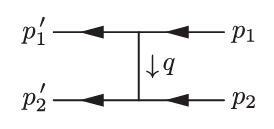
\includegraphics[width=0.7\textwidth]{4.png}
	\caption{two-nucleon-to-two-nucleon Feynman diagram}
\end{figure}
This is a diagram with 4 external lines.There exsits diagram having no external line in two-nucleon-to-two-nucleon order $\mathscr{O}(g^2)$ term:
\begin{figure}[htbp]
	\centering
	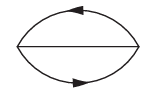
\includegraphics[width=0.7\textwidth]{5.png}
	\caption{diagram with no external lines}
\end{figure}

Since no external lines are in this diagram thus no momentum labelling.
\par There are also Feynman diagrams for renormalization terms,which obeys identical constructing rules as usual diagrams.Particularly,for vaccum counterterm,its diagram is a dot with a cross at it(no special meaning,just to make things better recognized).
\vspace{0.3\textheight}
\par Same as case in Wick's diagram,calculating S-matrix is nothing differnt from drawing and calculating Feynman diagrams.The rules follow which diagram transforms back to integral express are listed out:

\begin{figure}[htbp]
	\centering
	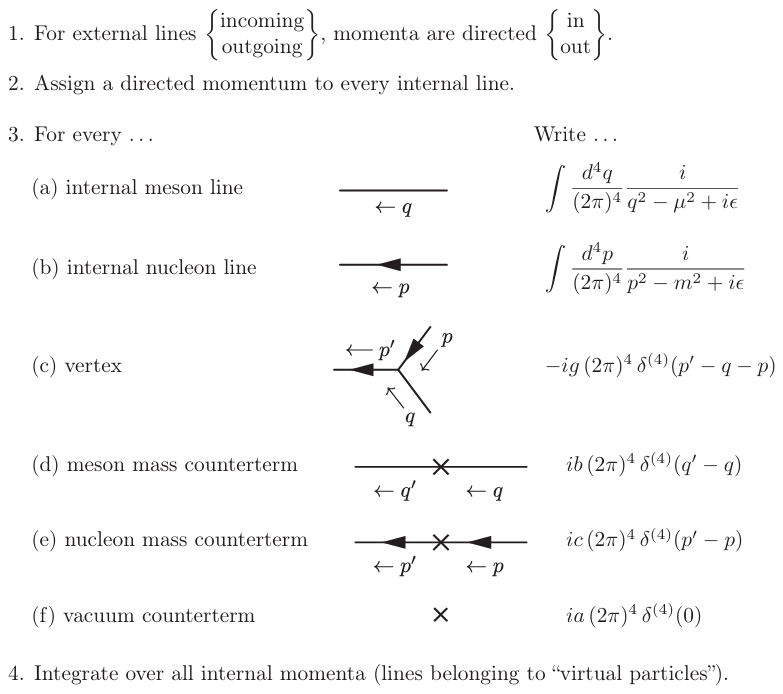
\includegraphics[width=0.85\textwidth]{6.png}
	\caption{Feynman rules for model 3}
\end{figure}

One can see a lot of delta functions and they're there to guaranteen conservation of momentum.Graphically speaking,for any vertex,the momentum flowing in must be equal to the momentum flowing out.
\section{a quick example}
two-nucleon-to-two-nucleon S-matrix to order $\mathscr{O}(g^2)$ can be easily calculated using Feynman diagram.For reaction $NN\rightarrow NN$,there are only two different Feynman diagrams (a),(b)
\begin{figure}[htbp]
	\centering
	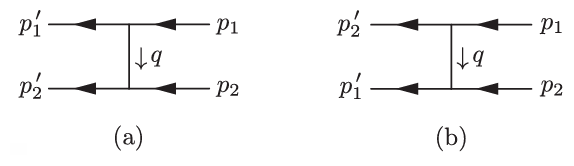
\includegraphics[width=0.7\textwidth]{7.png}
	\caption{two possible Feynman diagrams}
\end{figure}

According to rules,the integral form can be read out
\begin{align*}
	&\int\frac{d^4q}{(2\pi)^4}\frac{i}{q^2-m^2+i\epsilon}\times(-ig)(2\pi)^4\delta^{(4)}(q+p_1'-p_1)\\&\times(-ig)(2\pi)^4\delta^{(4)}(q+p_2'-p_2)+(p_1\leftrightarrow p_2)
\end{align*}
where $(p_1\leftrightarrow p_2)$ swaping $p_1$ and $p_2$ in the first term.Note that$$\delta(x-a)\delta(x-b)=\delta(a-b)\delta(x-a)=\delta(a-b)\delta(x-b)$$continue the calculation and find that the result$$-g^2[\frac{i}{(p_1-p_1')^2-m^2+i\epsilon}+\frac{i}{(p_1-p_2')^2-m^2+i\epsilon}]$$
elegant and simple.
\end{document}